% Electrical circuit
% Author: Stefan Kottwitz
% https://www.packtpub.com/hardware-and-creative/latex-cookbook
\documentclass[border=5pt]{standalone} 
%%%<
\usepackage{verbatim}
%%%>
\begin{comment}
:Title: Electrical circuit
:Tags: Electrics;Graphics;TikZ
:Author: Stefan Kottwitz
:Slug: circuits

Electrical documents, especially for learners, can contain a lot
of formulas. So LaTeX with its strengths in math typesetting is
a very good choice for writers. Electrical units are
easily written complying to standards using the siunitx package.

It seems natural, to also draw circuits directly within LaTeX.
In contrast to including external drawings, native LaTeX drawings
can have annotations which perfectly match the text,
with font and styles.

Here, we draw a circuit with common electrical components such as
a resistor, a diode, a capacitor, a bulb, and more. It shall be
a sample illustration, so don’t try building this one with
real components at home. ;-)

The TikZ package provides several libraries for drawing electrical
and logical circuits. We will choose one following the IEC norm.

The code is fully explained in the LaTeX Cookbook, Chapter 11,
Science and Technology, Drawing electrical circuits.
\end{comment}
\usepackage{tikz}
\usetikzlibrary{circuits.ee.IEC}
\begin{document}
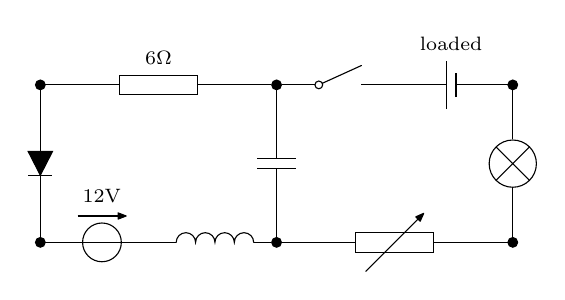
\begin{tikzpicture}[
    circuit ee IEC,
    x = 3cm, y = 2cm,
    every info/.style = {font = \scriptsize},
    set diode graphic = var diode IEC graphic,
    set make contact graphic = var make contact IEC graphic,
  ]
  \foreach \i in {1,...,3} {
    \node [contact] (lower contact \i) at (\i,0) {};
    \node [contact] (upper contact \i) at (\i,1) {};
  }
  \draw (upper contact 1) to [diode] (lower contact 1);
  \draw (lower contact 2) to [capacitor] (upper contact 2);
  \draw (upper contact 1) to [resistor = {ohm = 6}]
        (upper contact 2);
  \draw (lower contact 2) to [resistor = {adjustable}]
        (lower contact 3);
  \draw (lower contact 1) to [
           voltage source = {near start,
                             direction info = {volt = 12}},
           inductor = {near end}]
        (lower contact 2);
  \draw (upper contact 2) to [make contact = {near start},
                              battery = {near end,
                                         info = {loaded}}]
        (upper contact 3);
  \draw (lower contact 3) to [bulb = {minimum height = 0.6cm}]
        (upper contact 3);
\end{tikzpicture}
\end{document}

